
\documentclass{article}
\usepackage{graphicx}
\usepackage{amssymb}
\graphicspath{ {pictures/} }
\begin{document}

\title{Routing a Robot to Collect Data from $n$ Underwater Sensors in Minimum Time}
\author{Srikanth K.V.S., Aaron T.\ Becker}
\maketitle

\begin{figure}[htb]
\begin{center}
	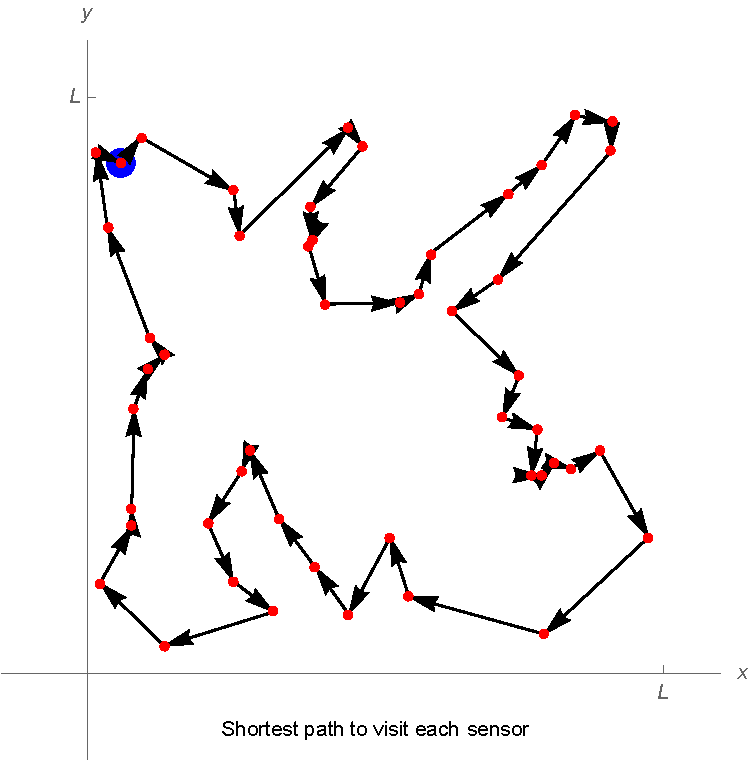
\includegraphics[width=0.48\columnwidth]{ShortestPathToSensors}
	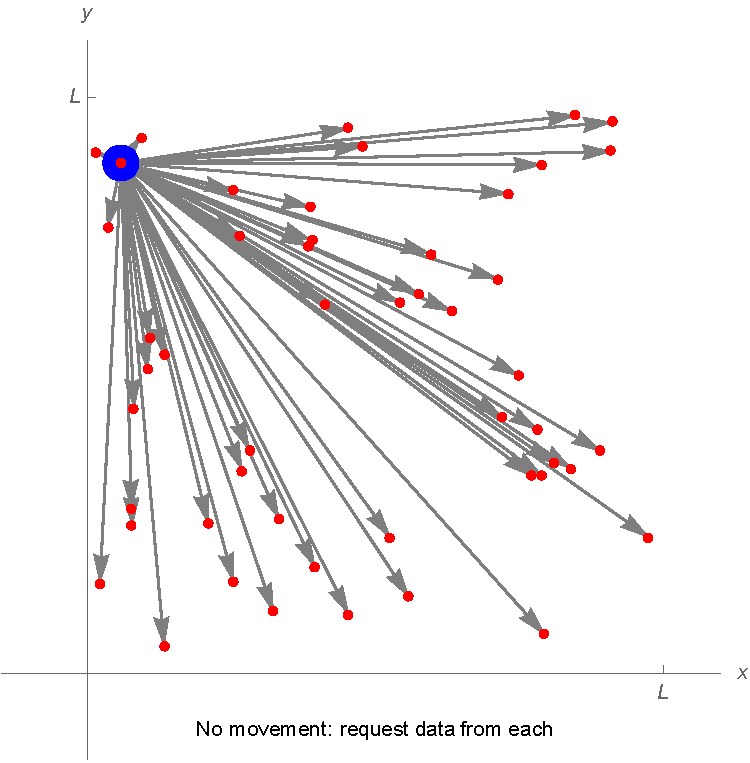
\includegraphics[width=0.48\columnwidth]{CommToEachSensor}
\end{center}
\caption{Data from $n$ nodes can be acquired by visiting each node, or by staying in place and communicating to each node.
\label{fig:ShortestPath}}
\end{figure}




\section{Introduction}

 Assume $n$ underwater sensor nodes must transmit data to a mobile underwater robot located at a depot, as illustrated in Fig.\ \ref{fig:ShortestPath}.  We wish to minimize the total time required to transmit this data to the depot. 
The robot could potentially shorten transmission time by moving towards nodes to increase data transmission rate.
This paper examines the motion-planning problem for a mobile robot to collect data from all nodes in minimum time.  
The path of a robot is defined by $N$ waypoints, starting at the depot, and returning to the depot, so waypoint 0 = waypoint $N+1$.
The $N$ waypoints are in $\mathbb{R}^3$. The robot travels along the straight line joining two waypoints. 
%The robot travels in closed paths to accomplish the task of collecting data hence has to traverse $N+1$ waypoints to complete a closed path. 
%The waypoint $N = 0$ will act as a depot for offloading the collected data and recharging.
The task is complete when the robot returns to the depot.


\section{Time for servicing $n$ sensor nodes (Moving)}

\begin{figure}[htb]
\begin{center}
	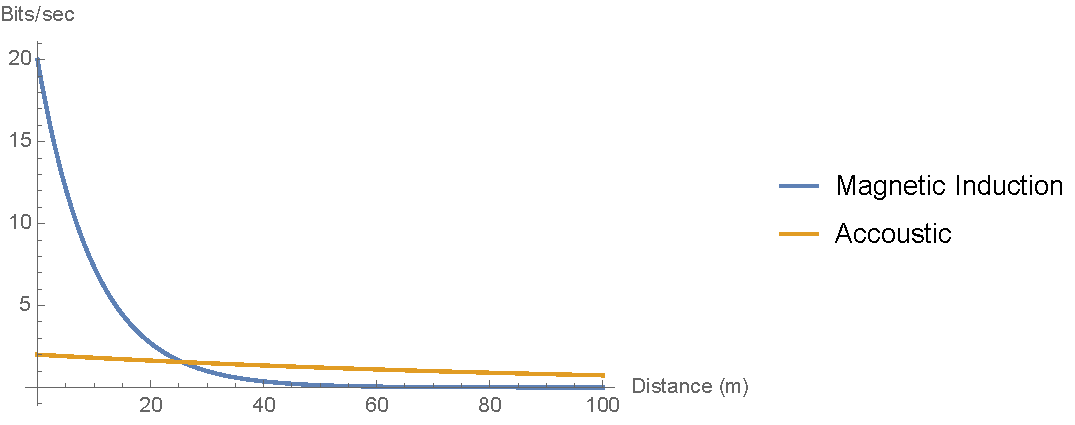
\includegraphics[width=0.8\columnwidth]{CommModel}
\end{center}
\caption{Two communications models, each based on exponential decay. 
\label{fig:CommModel}}
\end{figure}





 Data transmission can be performed by either \emph{magnetic induction communication} or \emph{acoustic communication}. 
 Both methods have their advantages and disadvantages.
Magnetic induction has higher bandwidth at close range, but bandwidth falls faster with increasing range.
Acoustic communication has lower bandwidth at close range, but bandwidth falls more slowly with increasing range.
This paper examines how to combine both to improve efficiency.
\\
\begin{center}
\begin{tabular}{ c l  c }
parameter & symbol  & units\\ 
\hline
Length of workspace side & $L$ & m\\
 Data Rate for Magnetic Induction & $ DR_{MI}(d)$  & b/s\\ 
 Data Rate for Acoustic  & $ DR_{Ac}(d)$ & b/s \\  
 Velocity of the robot & $ v$ & m/s \\ 
 Data stored in each sensor node   & $ Data_j$ & b\\
 Position of sensor $j$& $P_j$ & m, in $\mathbb{R}^3$\\
  Position of waypoint $i$ & $W_i$ & m, in $\mathbb{R}^3$\\
 \hline
\end{tabular}
\end{center}


\begin{equation}
    \label{TimeEqn_Moving}
   Time_{\textrm{visit each node}}  = \left [\frac{1}{v} \sum_{i=0}^{n+1} \left\| W_{i} - W_{i-1}\right\|_2 \right] +\left [\frac{1}{DR(d)} \sum_{j=1}^{n} Data_j\right]    
\end{equation}
The first term in equation 1 indicates\textbf{ travel time}.
The second term indicates the \textbf{transmission time}.


\label{Dist_Definition}
\begin{equation}
D_{ij} = \|W_{p}(i)-P_{j}\|
\end{equation}


For obtaining the solution we will use a TSP (Traveling Salesman Problem) solver.

\section{Time for servicing $n$ sensor nodes (Stationary)}

\begin{figure}[htb]
\begin{center}
	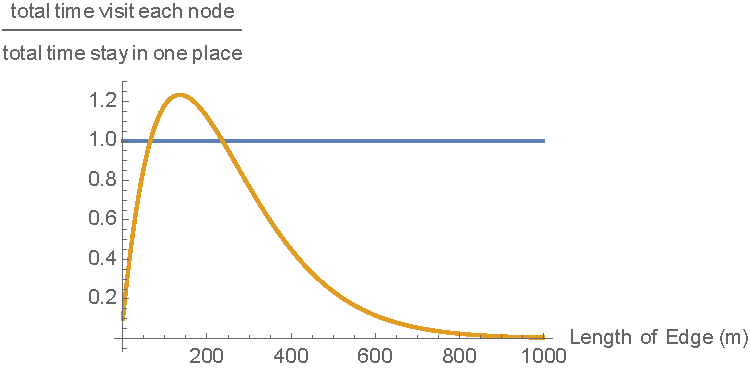
\includegraphics[width=0.8\columnwidth]{CompareVisitEachToComm}
\end{center}
\caption{ 
 The two techniques shown in Fig.\ \ref{fig:ShortestPath} have differing costs as a function of the length of the workspace edges.
\label{fig:CompareTwoPathTechniques}}
\end{figure}


\begin{equation}
    \label{TimeEqn_Stationary}
    Time_{\textrm{stay at depot}} = 0 + \sum_{i=1}^{n} \|P_{i}-P_{o}\| 
    \end{equation} 
\begin{equation}
    \label{Transmission}
    min_{(1/D.R_{MI})}*(Dist),min_{(1/D.R_{Ac})}*(Dist)  
\end{equation}
0 refers to the the traveling cost.\\*
The rest is the transmission cost.

\section{General Cost}
We assume that the robot can simultaneously receive both magnetic and acoustic transmissions, but only when the robot is not moving.
Given a path composed of $N$ waypoints, the minimum time solution is found by solving the following linear programming problem:
\label{GeneralCost_SingleMode}
\begin{equation}
1/v \sum_{i=0}^{N+1} \|W_{p}(i)-W_{p}(i-1)\|+\sum_{i=0}^{N}\sum_{j=1}^{n}  \frac{ a_{ij}}{DR(\|W_{p}(i)-P{j}\|_2)}
\end{equation}
with constraints:
\label{GeneralCostSingle_Constraints}
\begin{equation}
\sum_{i=0}^{N} a_{ij} = Data_j,~ \forall j \in [1,n], ~
 a_{ij}\geq 0
\end{equation}
The $a_{ij}$ parameters determine what fraction of sensor node $j$'s data should be transmitted at waypoint $i$.

If we have two communication modalities, the problem space is more rich, and is formulated as the linear programming problem:
\label{GeneralCost_DoubleMode}
\begin{equation}
1/v \sum_{i=0}^{n+1} \|W_{p}(i)-W_{p}(i-1)\|+\sum_{i=0}^{N}\sum_{j=1}^{n} \left(  \frac{ a_{ij}}{DR_{MI}(d_{ij})}  +  \frac{ b_{ij}}{DR_{Ac}(d_{ij})}  \right)
\end{equation}
with constraints:
\label{GeneralCostDouble_Constraints}
\begin{equation}
\sum_{i=0}^{N} a_{ij}+b_{ij}=Data_j, ~\forall j \in [1,n], ~
 a_{ij}\geq 0,b_{ij}\geq 0
\end{equation}

here, $a_{ij}$ parameters determine what fraction of sensor node $j$'s data should be transmitted at waypoint $i$ using magnetic induction, while $b_{ij}$ is for acoustic.

bits transmitted from sensor at  location $s$, $(xy)$ is $(sx,sy)$ when vehicle is 
moving at velocity $v$ between $p1$  $(p_{1}^{x},p_{1}^{y})$ and $p2$  $(p_{2}^{x},p_{2}^{y})$ is : 
\label{Drive_and_Transmit}
\begin{equation}
(Sqrt[(p1x - p2x)^2 + (p1y - p2y)^2]/v)* Integrate[e^(-Sqrt[(p1x + (p2x - p1x)*p - sx)^2+ (p1y + (p2y - p1y)*p - sy)^2]), {p, 0, 1}]
\end{equation}
The first term is  a constant:  distanct/velocity:
\label{Drive_and_Transmit_constant}
\begin{equation}
(Sqrt[(p1x - p2x)^2 + (p1y - p2y)^2]/v)
\end{equation}
The next term is an integral from p = 0 to p = 1  (p is progress along straight line from p1 to p2:
\label{Drive_and_Transmit_integral}
\begin{equation}
e^(-Sqrt[(p1x + (p2x - p1x)*p - sx)^2+ (p1y + (p2y - p1y)*p - sy)^2])
\end{equation}
e  is the base of the natural logarithm.
\end{document}
